\documentclass[conference]{IEEEtran}
\usepackage{graphicx}
\usepackage{booktabs}
\usepackage{amsmath}
\usepackage{multirow}
\usepackage{xcolor}
\usepackage{url}
\usepackage{listings}
\lstset{basicstyle=\ttfamily\scriptsize, columns=fullflexible, frame=single,
        keywordstyle=\bfseries, language=Verilog, breaklines=true}
\graphicspath{{figures/}{diagrams/}}
% ---- fill in before submission --------------------------------------------
\newcommand{\memberA}{Arya Pandey}
\newcommand{\memberB}{Divyansh Rathore}
\newcommand{\memberC}{Rishita Boisnobi}
\newcommand{\memberD}{Mohit Singh}
\newcommand{\memberE}{Abhishek Sharma}
\newcommand{\institute}{NST\\ RU, Sonipat, Haryana, India}
% ---------------------------------------------------------------------------

\begin{document}

\title{Design and FPGA Implementation of a Parameterised\\ Systolic-Array Matrix-Multiplication Accelerator}

\author{
\IEEEauthorblockN{\memberA, \memberB, \memberC, \memberD, \memberE}
\IEEEauthorblockA{\institute}
}

\maketitle

% =====================================================================
\begin{abstract}
Matrix multiplication dominates the run time of neural-network inference and
many signal-processing kernels. This paper presents the design, verification
and FPGA implementation of a compact, parameterised output-stationary systolic
array that multiplies two $N\times N$ signed 8-bit fixed-point (Q4.4) matrices.
The accelerator is written in synthesizable Verilog-2001 with a modular
hierarchy: multiply-accumulate (MAC) unit, processing element (PE), $N\times N$
PE grid, skewing input buffers, an output capture buffer, a finite-state-machine
controller and a simple memory-mapped matrix data interface. A cycle-accurate
Python reference model generates fourteen directed and random test cases per
array size; all of them pass for $N=3$, 4 and 8 in Icarus Verilog
simulation. A $4\times4$ array completes one multiplication in 14 clock
cycles from \textit{start} to \textit{done} (compute latency $3N-1=11$ cycles)
against 67 cycles for a single-MAC sequential baseline, a $4.8\times$ cycle
speed-up that grows to $19.8\times$ at $N=8$. Post-route on a Lattice iCE40-HX8K
the array closes timing at 79.2\,MHz (baseline 58.1\,MHz), giving a
$6.5\times$ wall-clock speed-up and a $1.6\times$ better area--delay product.
Mapped to a Xilinx Artix-7, the $4\times4$ array uses 16 DSP48E1 slices,
137 LUTs and 456 flip-flops.
\end{abstract}

\begin{IEEEkeywords}
Systolic array, matrix multiplication, hardware accelerator, multiply-accumulate,
FPGA, fixed-point arithmetic, Verilog, AI acceleration.
\end{IEEEkeywords}

% =====================================================================
\section{Introduction}
General matrix multiplication (GEMM) accounts for the overwhelming majority of
arithmetic in convolutional and transformer neural networks, which is why
accelerators from mobile NPUs to Google's Tensor Processing Unit (TPU) are built
around dense MAC arrays~\cite{jouppi2017tpu,sze2017efficient}. A general-purpose
processor executes the $N^3$ multiply-accumulates of an $N\times N$ product
largely sequentially and spends most of its energy moving operands between
memory and registers. A \emph{systolic array}~\cite{kung1979systolic,kung1982why}
instead arranges many simple PEs in a regular grid in which data is pumped
rhythmically from neighbour to neighbour, so that every operand fetched from
memory is reused $N$ times and all PEs work in parallel using only local,
short wires.

The objective of this project is to design such an array at a scale suitable
for an undergraduate FPGA project, to verify it rigorously against a software
reference model, and to quantify its benefit over a sequential multiplier in
terms of latency, throughput, clock frequency and FPGA resources. The
contributions of Phase~I are:
\begin{itemize}
  \item a fully parameterised ($N$, data width, accumulator width) Verilog
        RTL of an output-stationary systolic array with a complete control and
        host-interface path;
  \item a sequential single-MAC baseline with an identical interface, enabling
        like-for-like comparison;
  \item a self-checking verification environment (unit tests for the MAC and
        PE, and a matrix-level testbench driven by a Python golden model);
  \item open-source synthesis and place-and-route results with cycle,
        throughput and resource analysis for $N\in\{2,3,4,8\}$.
\end{itemize}

% =====================================================================
\section{Literature Review}
\textbf{Systolic arrays.} Kung and Leiserson introduced systolic arrays for
VLSI in 1978 as a way to map regular algorithms such as matrix multiplication,
convolution and LU decomposition onto arrays of identical cells with nearest-neighbour
communication~\cite{kung1979systolic}. Kung later argued that their key virtue
is balancing computation against I/O bandwidth: each datum entering the array
is used many times~\cite{kung1982why}. S.~Y.~Kung's text~\cite{kung1988vlsi}
formalised space--time mapping of algorithms onto such arrays, including the
\emph{output-stationary}, \emph{weight-stationary} and \emph{input-stationary}
dataflows.

\textbf{Modern DNN accelerators.} Google's first-generation TPU uses a
$256\times256$ weight-stationary systolic array of 8-bit MACs and delivers
92\,TOPS, $15$--$30\times$ faster than contemporary CPUs/GPUs on inference
workloads~\cite{jouppi2017tpu}. Eyeriss~\cite{chen2017eyeriss} proposed a
row-stationary dataflow on a $12\times14$ PE array to minimise data movement
energy for convolutions, and Sze \emph{et al.}~\cite{sze2017efficient} survey
how the choice of dataflow trades storage, reuse and bandwidth. Gemmini~\cite{genc2021gemmini}
is an open-source, parameterised systolic-array generator integrated with a
RISC-V SoC that supports both output- and weight-stationary modes, and
SCALE-Sim~\cite{samajdar2018scale} is an analytical simulator for exploring
array size and dataflow trade-offs.

\textbf{Fixed-point arithmetic.} Jacob \emph{et al.}~\cite{jacob2018quantization}
showed that 8-bit integer arithmetic with wide (32-bit) accumulators preserves
accuracy for CNN inference, motivating narrow operands and a wide
accumulator, which we adopt here at a reduced scale (8-bit operands, 20-bit
accumulator).

\textbf{FPGA implementation.} On Xilinx 7-series devices, a signed
$25\times18$ multiplier and 48-bit accumulator are available in each DSP48E1
slice~\cite{ug479}, so one PE maps naturally to one DSP. Open-source flows
based on Yosys and nextpnr~\cite{shah2019yosys} now provide complete
synthesis and timing-driven place-and-route for Lattice iCE40/ECP5 devices,
which we use alongside Yosys' Xilinx mapping.

\textbf{Gap addressed.} Industrial accelerators are far too large to study at
RTL in a semester. This work isolates the essential mechanism---skewed operand
injection, nearest-neighbour forwarding and in-place accumulation---in a small,
readable and fully verified design, and measures its benefit against a
sequential baseline under the same interface.

% =====================================================================
\section{Proposed Solution}

\subsection{System Architecture}
Fig.~\ref{fig:block} shows the top-level architecture
(\texttt{systolic\_top}). The host writes the elements of $A$ and $B$ into two
\texttt{input\_buffer}s through the matrix data interface, then pulses
\texttt{start}. The \texttt{systolic\_controller} clears the array and steps a
counter $t$ that drives both buffers. The A buffer feeds row $i$ of $A$ into the
left edge of PE row $i$; the B buffer feeds column $j$ of $B$ into the top edge
of PE column $j$. Each PE multiplies the two operands passing through it, adds
the product to its local accumulator, and forwards $a$ to the right and $b$
downwards. When the last operand pair has reached PE$_{N-1,N-1}$, the
controller copies all $N^2$ accumulators into the \texttt{output\_buffer}, from
which the host reads $C$.

\begin{figure*}[t]
  \centering
  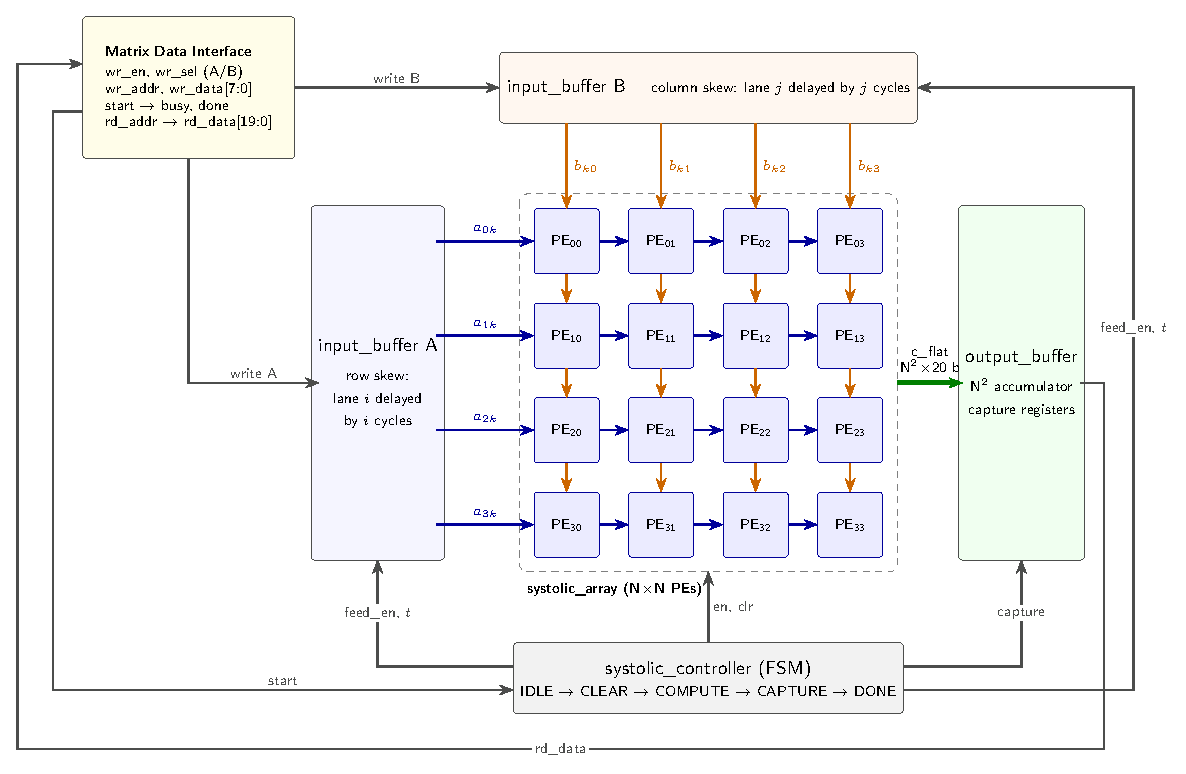
\includegraphics[width=0.86\textwidth]{block_diagram.pdf}
  \caption{Architecture of the $4\times4$ output-stationary systolic-array
  accelerator (module names as in the RTL).}
  \label{fig:block}
\end{figure*}

The RTL hierarchy is:
\begin{lstlisting}
systolic_top
 |- systolic_controller  (FSM, step counter)
 |- input_buffer  u_buf_a (A storage + row skew)
 |- input_buffer  u_buf_b (B storage + col skew)
 |- systolic_array       (N x N generate grid)
 |    '- pe  x N^2       (forward regs + MAC)
 |         '- mac_unit
 '- output_buffer        (N^2 capture regs)
seq_matmul               (baseline, same ports)
\end{lstlisting}

\subsection{Number Format and MAC Unit}
Operands are 8-bit two's-complement numbers interpreted as Q4.4 (range
$[-8, 7.9375]$, resolution $1/16$). Their product is exact in 16 bits (Q8.8)
and is sign-extended into a 20-bit accumulator (Q12.8). Since
$|a\cdot b|\le 2^{14}$, the accumulator can absorb $2^{19}/2^{14}=32$
worst-case products without overflow, which covers $N\le 32$; no rounding or
saturation is therefore needed for the sizes studied. The \texttt{mac\_unit}
implements
\begin{equation}
acc \leftarrow
\begin{cases}
0 & \text{clr}\\
a\cdot b & \text{en}\wedge\text{load}\\
acc + a\cdot b & \text{en}\\
acc & \text{otherwise.}
\end{cases}
\end{equation}

\subsection{Processing Element}
The PE (Fig.~\ref{fig:pe}) contains the MAC unit plus two 8-bit pipeline
registers that forward $a_{in}\to a_{out}$ and $b_{in}\to b_{out}$ with one
cycle of latency. A global enable allows the whole array to be stalled, and a
synchronous clear zeroes the accumulators and flushes the pipeline registers
before each job. Because the result stays in the PE until it is complete, this
is an \emph{output-stationary} dataflow.

\begin{figure}[t]
  \centering
  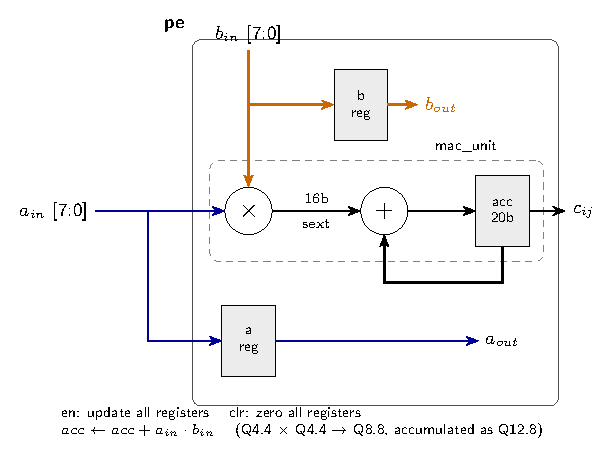
\includegraphics[width=0.92\columnwidth]{pe_micro.pdf}
  \caption{Processing element micro-architecture.}
  \label{fig:pe}
\end{figure}

\subsection{Systolic Data Movement and Skew}
For PE$_{ij}$ to multiply matching operands $a_{ik}$ and $b_{kj}$, row $i$ of $A$
is delayed by $i$ cycles and column $j$ of $B$ by $j$ cycles. The input buffer
implements this skew directly from its storage: at step $t$ lane $l$ outputs
\begin{equation}
a\text{-lane}_l(t) = A[l][t-l],\qquad b\text{-lane}_l(t) = B[t-l][l]
\end{equation}
when $0\le t-l<N$, and zero otherwise. Zero is the neutral element of the MAC,
so PEs run unconditionally without per-PE valid logic. With the registered
buffer output and one hop per PE, operand pair $(a_{ik},b_{kj})$ meets in PE$_{ij}$
in compute cycle
\begin{equation}
\tau_{ijk} = i + j + k + 1 .
\end{equation}
The last pair ($i=j=k=N-1$) arrives in cycle $3N-2$, so the compute phase lasts
$3N-1$ cycles. Fig.~\ref{fig:dataflow} illustrates the resulting diagonal
wavefront for $N=3$.

\begin{figure*}[t]
  \centering
  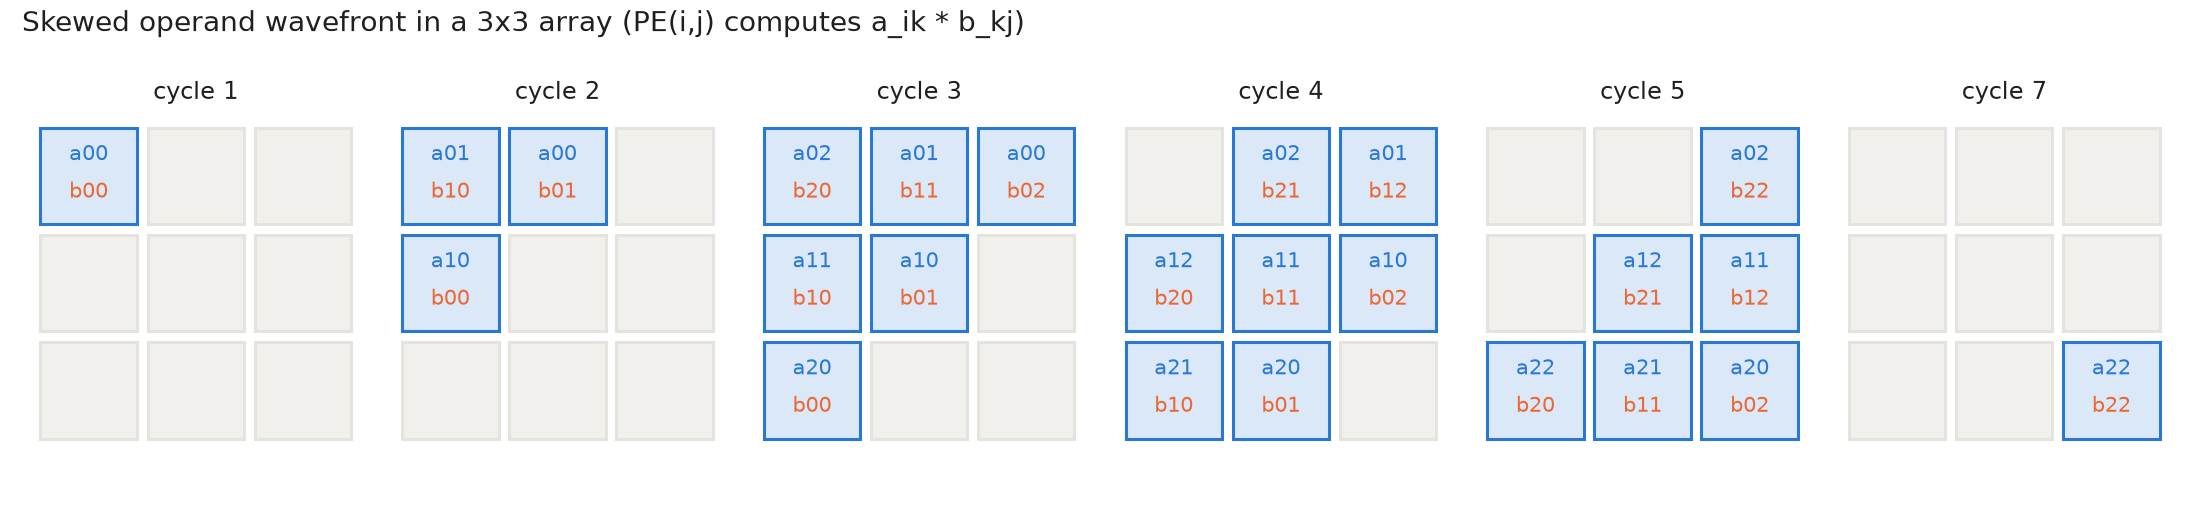
\includegraphics[width=0.95\textwidth]{dataflow_skew.png}
  \caption{Operand wavefront in a $3\times3$ array: in each cycle, PE$_{ij}$
  holds $a_{ik}$ (blue) and $b_{kj}$ (orange) with $k=\tau-1-i-j$.}
  \label{fig:dataflow}
\end{figure*}

\subsection{Controller}
The Moore FSM of Fig.~\ref{fig:fsm} sequences one job:
IDLE $\rightarrow$ CLEAR (1 cycle, \texttt{clr}) $\rightarrow$ COMPUTE
($3N-1$ cycles, \texttt{en}, \texttt{feed\_en}, $t=0\ldots3N-2$) $\rightarrow$
CAPTURE (1 cycle) $\rightarrow$ DONE (1-cycle \texttt{done} pulse). Including
the cycle in which \texttt{start} is sampled, the start-to-done latency is
$3N+2$ cycles. Writes to the buffers are blocked while \texttt{busy} is high.

\begin{figure}[t]
  \centering
  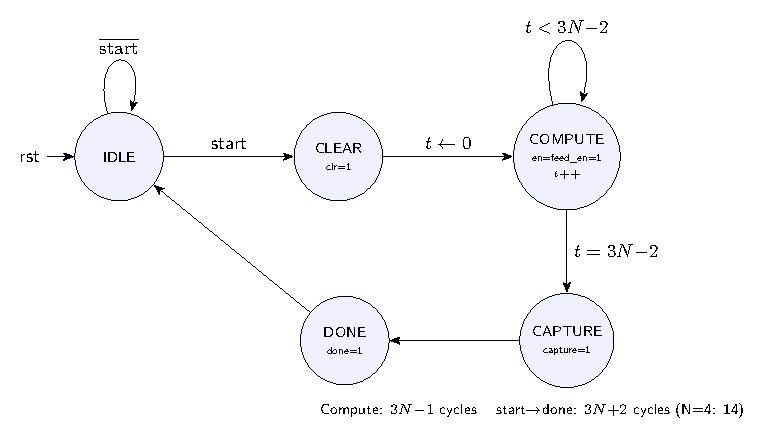
\includegraphics[width=0.95\columnwidth]{fsm.pdf}
  \caption{State-transition diagram of \texttt{systolic\_controller}.}
  \label{fig:fsm}
\end{figure}

\subsection{Matrix Data Interface}
The host side is a simple synchronous SRAM-like port:
\texttt{wr\_en}, \texttt{wr\_sel} (0\,=\,A, 1\,=\,B), \texttt{wr\_addr}
($=\text{row}\cdot N+\text{col}$), \texttt{wr\_data[7:0]}; \texttt{start},
\texttt{busy}, \texttt{done}; and a combinational read port
\texttt{rd\_addr}\,$\rightarrow$\,\texttt{rd\_data[19:0]}. The port is deliberately
narrow (one element per cycle) so that it can be driven by a UART bridge or a
soft processor in Phase~II.

\subsection{Baseline: Sequential Multiplier}
\texttt{seq\_matmul} has exactly the same ports but a single MAC unit that
iterates over $(i,j,k)$. The \texttt{load} input of the MAC starts each new dot
product, and the previous result is written back to the result memory in the
same cycle, so the design needs $N^3$ MAC cycles plus one flush cycle
($N^3+3$ cycles start-to-done).

% =====================================================================
\section{Verification Methodology}
A Python/NumPy golden model generates, for each $N$, fourteen test cases and
their exact integer products, stored as \texttt{\$readmemh} hex files
(Table~\ref{tab:tests}). Three self-checking testbenches are run in Icarus
Verilog~\cite{icarus}:
\begin{itemize}
\item \texttt{tb\_mac\_unit}: 13 directed checks---signed products, enable
      hold, load/clear priority, extreme operands ($127$, $-128$), 16
      worst-case accumulations without overflow, and a Q4.4 example
      ($1.5\times-2.25=-3.375$).
\item \texttt{tb\_pe}: 7 checks of one-cycle forwarding, stall, clear, a
      4-term dot product and insensitivity to zero bubbles.
\item \texttt{tb\_matmul}: loads every test through the host interface,
      measures start-to-done cycles, reads back all $N^2$ results and compares
      them to the model. The same bench drives the baseline when compiled with
      \texttt{-DSEQ}.
\end{itemize}

\begin{table}[t]
\centering
\caption{Matrix-level test cases (each run for $N=3,4,8$)}
\label{tab:tests}
\begin{tabular}{@{}cl@{}}
\toprule
\# & Purpose \\ \midrule
0, 1 & $I\times B$ and $A\times I$ (data routing) \\
2 & zero matrix $\times$ random \\
3--5 & all $+127$, all $-128$, $+127\times-128$ (range) \\
6 & $A=[1..N^2]$, $B=A^\mathsf{T}$ (ordering) \\
7 & Q4.4 fractional values (fixed-point) \\
8--13 & uniformly random signed 8-bit \\ \bottomrule
\end{tabular}
\end{table}

All waveforms are dumped to VCD and inspected in GTKWave;
Fig.~\ref{fig:wave} is rendered from the $4\times4$ VCD for test~0. It shows
the controller states, the skew (lane~3 of each buffer starts three cycles
after lane~0), and the order in which PEs complete: PE$_{00}$ in cycle~4,
PE$_{11}$ in cycle~7 and PE$_{33}$ in cycle~13, just before CAPTURE.

\begin{figure*}[t]
  \centering
  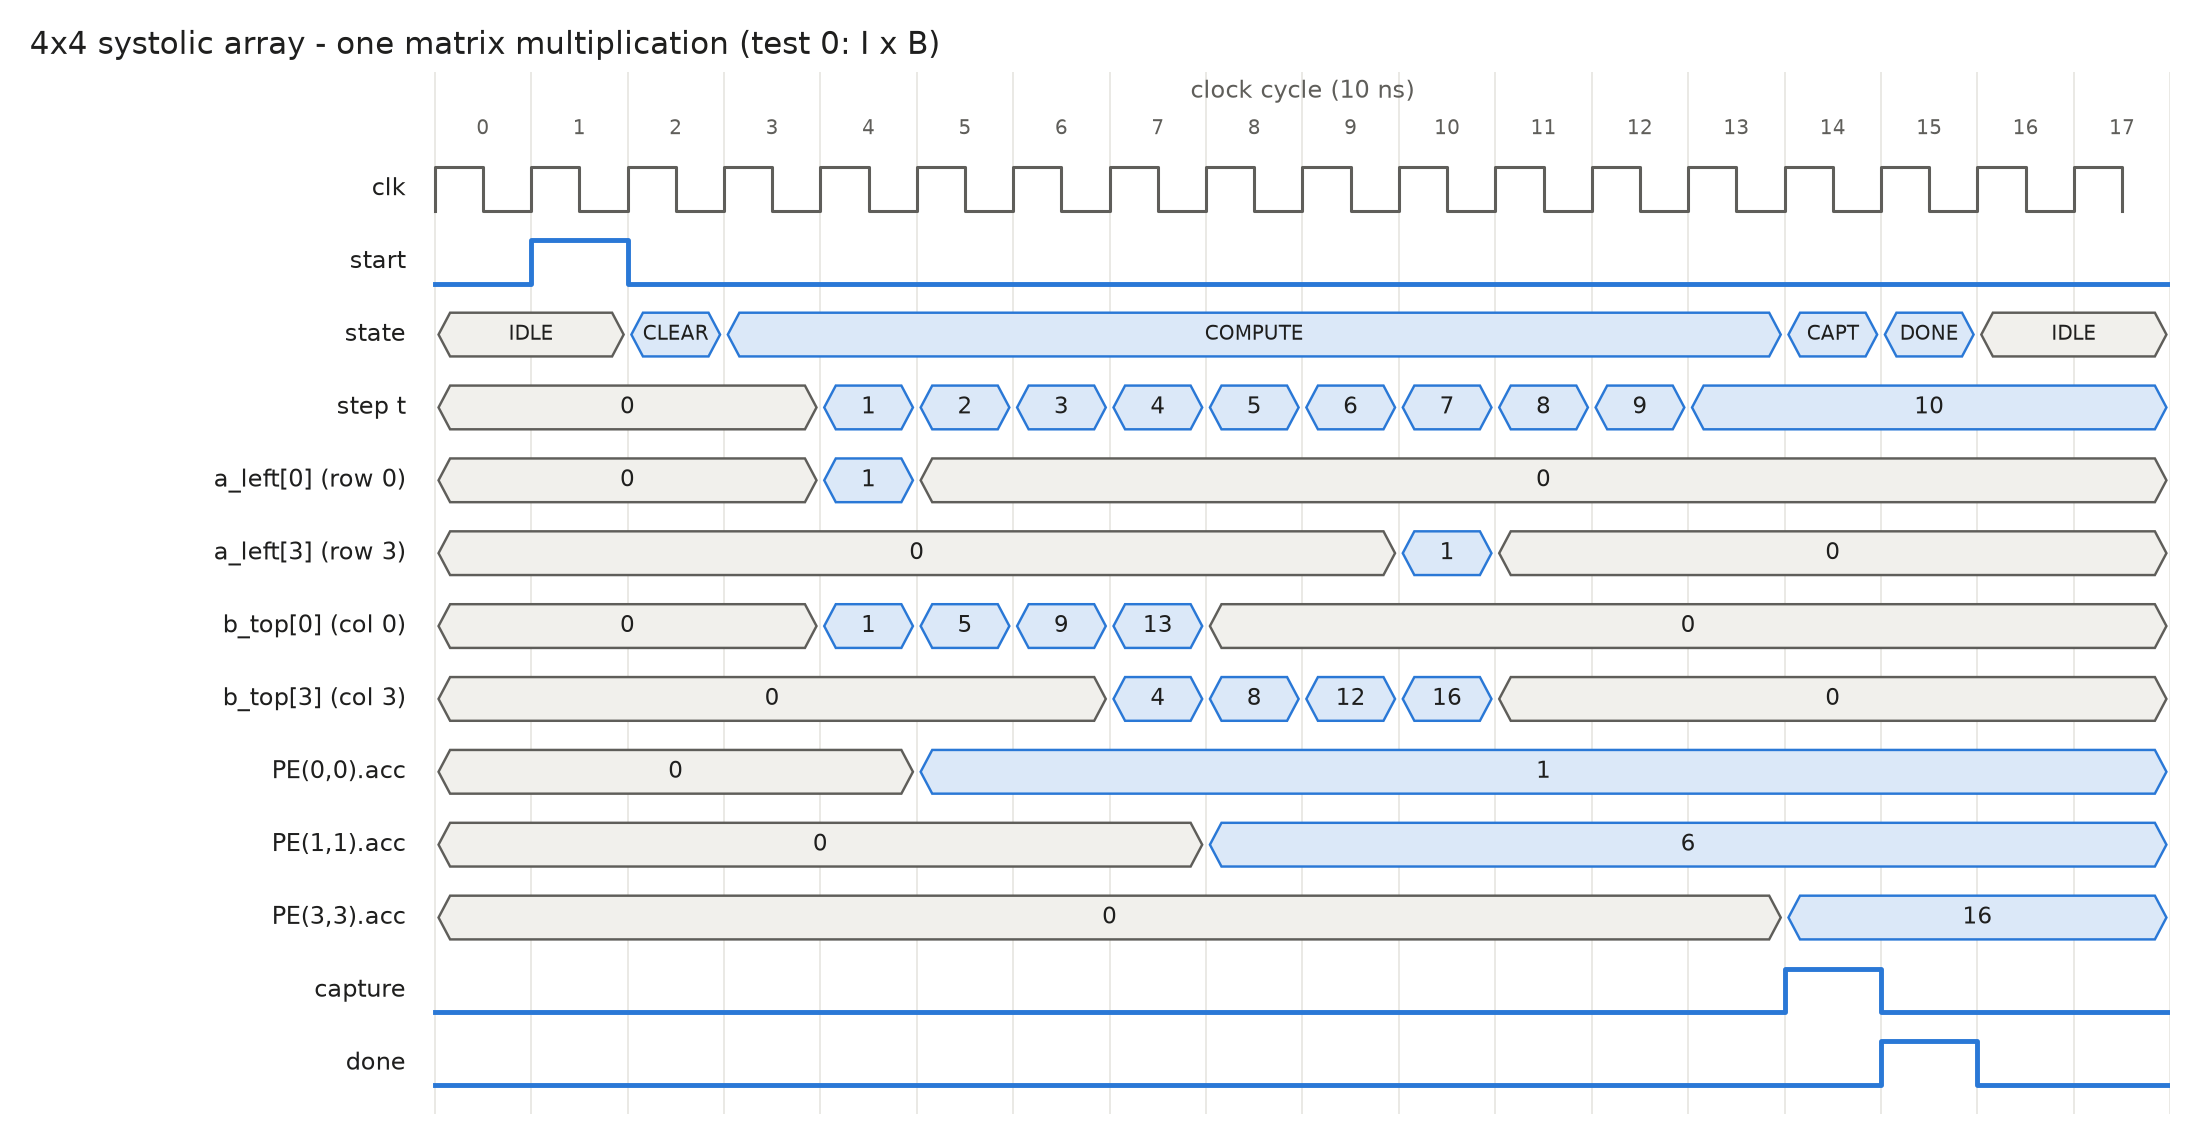
\includegraphics[width=0.9\textwidth]{waveform_systolic_N4.png}
  \caption{Simulated waveform of one $4\times4$ multiplication ($I\times B$,
  $B=[1..16]$). Values are signed decimal.}
  \label{fig:wave}
\end{figure*}

% =====================================================================
\section{Results}

\subsection{Functional Results}
All checks pass: 13/13 MAC, 7/7 PE, and $14/14$ matrix tests for each of
$N=3,4,8$ on both the systolic array and the baseline (84 matrix
multiplications, 0 mismatches). For test~7 ($N=4$) the array returns, e.g.,
$C_{00}=64$ (0.25 in Q12.8) and $C_{03}=-896$ ($-3.5$), identical to the model.

\subsection{Latency and Throughput}
Table~\ref{tab:perf} lists the measured start-to-done latencies. The systolic
latency grows linearly ($3N+2$) whereas the baseline grows cubically
($N^3+3$), Fig.~\ref{fig:lat}. Defining throughput as MACs completed per
cycle for a single job, the $4\times4$ array achieves $64/14=4.57$ MAC/cycle
vs.\ $0.96$ for the baseline. At the post-route clock this is
$362$\,MMAC/s ($0.72$\,GOPS) vs.\ $55.5$\,MMAC/s.

\begin{table}[t]
\centering
\caption{Measured latency (cycles, start$\rightarrow$done)}
\label{tab:perf}
\begin{tabular}{@{}lrrrr@{}}
\toprule
 & $N=2$ & $N=3$ & $N=4$ & $N=8$ \\ \midrule
Systolic ($3N{+}2$)   & 8  & 11 & 14 & 26 \\
Sequential ($N^3{+}3$) & 11 & 30 & 67 & 515 \\
Cycle speed-up        & 1.4$\times$ & 2.7$\times$ & 4.8$\times$ & 19.8$\times$ \\
Time @ iCE40 $f_{max}$ (ns), sys. & 92 & 133 & 177 & -- \\
Time @ iCE40 $f_{max}$ (ns), seq. & 177 & 524 & 1154 & -- \\
Wall-clock speed-up   & 1.9$\times$ & 3.9$\times$ & 6.5$\times$ & -- \\ \bottomrule
\end{tabular}
\end{table}

\begin{figure}[t]
  \centering
  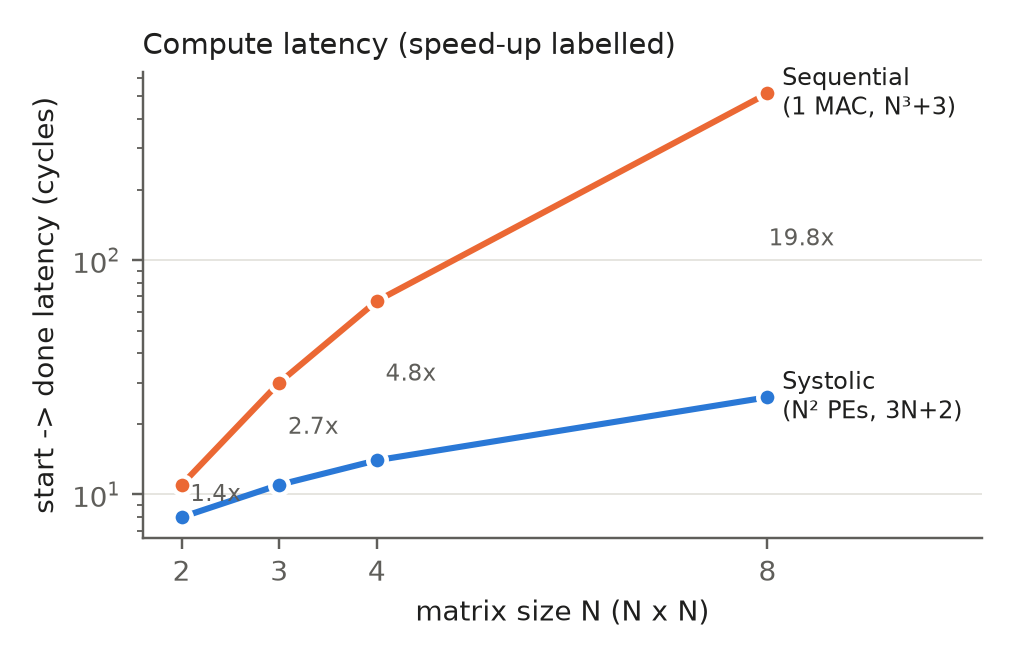
\includegraphics[width=0.95\columnwidth]{latency_vs_n.png}
  \caption{Latency vs.\ matrix size (log scale); labels give the speed-up.}
  \label{fig:lat}
\end{figure}

\subsection{Synthesis: Resources and Maximum Frequency}
Table~\ref{tab:synth} summarises synthesis. Xilinx figures are from Yosys
\texttt{synth\_xilinx -family xc7} (pre-placement estimate). iCE40 figures are
post-route from nextpnr-ice40 on an HX8K, which has no hard multipliers, so the
16 multipliers are built from LUTs and dominate the logic-cell count. On
Artix-7 each PE maps to exactly one DSP48E1 and the 20-bit accumulator is
absorbed into the DSP's internal P register, which is why the flip-flop count
is lower than the $N^2\times(20+16)$ bits one might expect. A $4\times4$ array
uses 18\,\% of the DSPs of the smallest Artix-7 on a Basys-3 board
(XC7A35T: 90 DSP48E1, 20\,800 LUTs).

\begin{table}[t]
\centering
\caption{Synthesis results}
\label{tab:synth}
\setlength{\tabcolsep}{4pt}
\begin{tabular}{@{}lcrrrrr@{}}
\toprule
& & \multicolumn{3}{c}{Artix-7 (Yosys)} & \multicolumn{2}{c}{iCE40-HX8K (P\&R)} \\
\cmidrule(lr){3-5}\cmidrule(lr){6-7}
Design & $N$ & LUT & FF & DSP & LCs & $f_{max}$ (MHz) \\ \midrule
Systolic   & 2 & 38  & 119  & 4  & 1314 & 86.8 \\
Systolic   & 3 & 90  & 236  & 9  & 3051 & 82.8 \\
Systolic   & 4 & 137 & 456  & 16 & 5430 & 79.2 \\
Systolic   & 8 & 500 & 2057 & 64 & --   & --   \\ \midrule
Sequential & 3 & 72  & 36   & 1  & 893  & 57.2 \\
Sequential & 4 & 59  & 36   & 1  & 1360 & 58.1 \\ \bottomrule
\end{tabular}
\end{table}

\textbf{Critical path.} In the systolic array, the post-route critical path on
iCE40 runs from a PE forwarding register through the LUT multiplier and
accumulator adder back into the accumulator (12.6\,ns). It is entirely local
to one PE, so $f_{max}$ degrades only slightly as $N$ grows
(86.8$\rightarrow$79.2\,MHz from $N=2$ to 4), mostly due to routing
congestion. The baseline is \emph{slower} (58\,MHz) because its operand path
passes through wide $N^2$:1 read multiplexers of the operand memories before
the multiplier---a concrete illustration of the systolic principle of local
communication.

\begin{figure}[t]
  \centering
  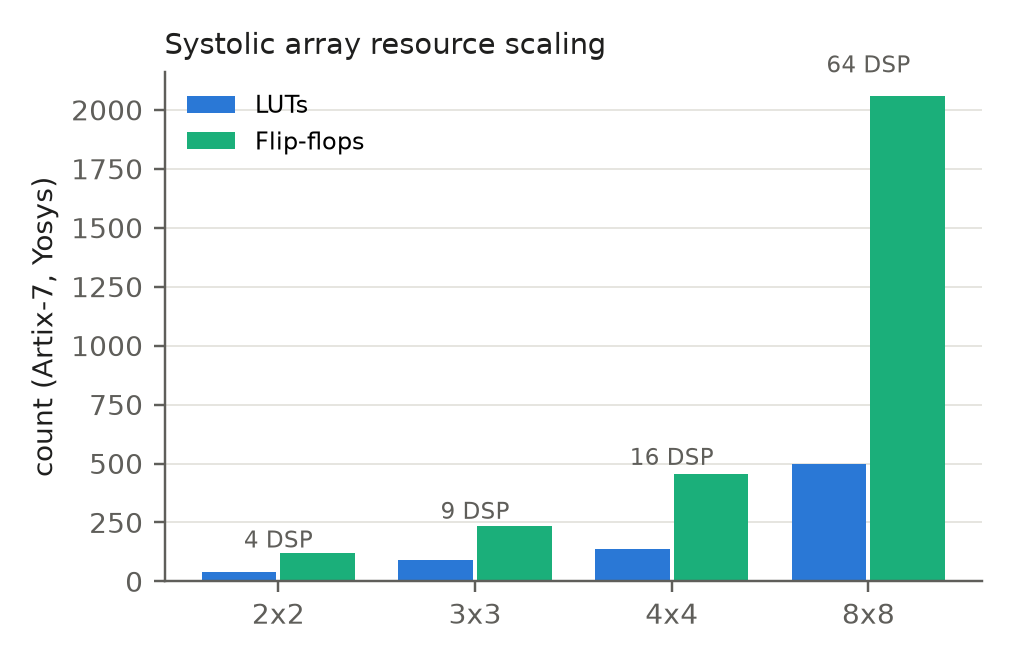
\includegraphics[width=0.95\columnwidth]{resources_vs_n.png}
  \caption{Systolic-array resource scaling on Artix-7.}
  \label{fig:res}
\end{figure}

\subsection{Comparison and Discussion}
\textbf{Area--delay.} On iCE40 the $4\times4$ array costs $4.0\times$ the
logic cells of the baseline but finishes $6.5\times$ sooner, giving a
$1.64\times$ better area--delay product
($5430\cdot177$ vs.\ $1360\cdot1154$ LC$\cdot$ns).

\textbf{PE utilisation.} A single job keeps the $N^2$ PEs busy for only
$N^3/(N^2(3N-1)) = 36\,\%$ of the compute cycles at $N=4$, because of the
fill and drain of the skewed wavefront. Overlapping consecutive jobs (starting
the next operands while the previous wavefront drains) would approach the
peak of $N^2=16$ MAC/cycle, i.e.\ 1.27\,GMAC/s at 79\,MHz.

\textbf{I/O bound.} Including the 32-cycle load and 16-cycle read of the
one-element-per-cycle host port, end-to-end time is 62 cycles for the array
vs.\ 115 for the baseline, only $1.85\times$ faster. As Kung
observed~\cite{kung1982why}, the array is fast enough that bandwidth becomes the
bottleneck; widening the interface to one row per cycle is a Phase~II goal.

% =====================================================================
\section{Individual Contributions}
The Phase~I work was divided as follows:
\begin{itemize}
\item \textbf{\memberA}: PE and MAC unit RTL, unit-level testbenches, fixed-point number format.
\item \textbf{\memberB}: systolic-array grid, input skew buffers and output buffer.
\item \textbf{\memberC}: controller FSM, matrix data interface and sequential baseline.
\item \textbf{\memberD}: Python reference model, matrix-level testbench and waveform analysis.
\item \textbf{\memberE}: synthesis and timing flow, performance analysis, report and video.
\end{itemize}

% =====================================================================
\section{Conclusion and Future Work}
A parameterised output-stationary systolic array for signed fixed-point matrix
multiplication was designed, verified against a golden model for $N=3,4,8$, and
synthesised for Xilinx and Lattice FPGAs. The $4\times4$ instance computes a
product in 14 cycles at 79\,MHz, $6.5\times$ faster than a sequential MAC
design, with only local interconnect on its critical path. Phase~II will
(i)~run the Vivado flow (\texttt{synth/vivado\_synth.tcl}) and demonstrate the
design on an Artix-7 board with a UART host link, (ii)~pipeline back-to-back
jobs to raise PE utilisation, (iii)~widen the data interface, and (iv)~tile
larger matrices over the $4\times4$ array.

% =====================================================================
\begin{thebibliography}{10}
\bibitem{kung1979systolic}
H.~T. Kung and C.~E. Leiserson, ``Systolic arrays (for VLSI),'' in
\emph{Sparse Matrix Proceedings 1978}, SIAM, 1979, pp.~256--282.

\bibitem{kung1982why}
H.~T. Kung, ``Why systolic architectures?'' \emph{Computer}, vol.~15, no.~1,
pp.~37--46, Jan. 1982.

\bibitem{kung1988vlsi}
S.~Y. Kung, \emph{VLSI Array Processors}. Englewood Cliffs, NJ, USA:
Prentice Hall, 1988.

\bibitem{jouppi2017tpu}
N.~P. Jouppi \emph{et al.}, ``In-datacenter performance analysis of a tensor
processing unit,'' in \emph{Proc. 44th Annu. Int. Symp. Computer Architecture
(ISCA)}, 2017, pp.~1--12.

\bibitem{chen2017eyeriss}
Y.-H. Chen, T.~Krishna, J.~S. Emer, and V.~Sze, ``Eyeriss: An energy-efficient
reconfigurable accelerator for deep convolutional neural networks,''
\emph{IEEE J. Solid-State Circuits}, vol.~52, no.~1, pp.~127--138, Jan. 2017.

\bibitem{sze2017efficient}
V.~Sze, Y.-H. Chen, T.-J. Yang, and J.~S. Emer, ``Efficient processing of deep
neural networks: A tutorial and survey,'' \emph{Proc. IEEE}, vol.~105, no.~12,
pp.~2295--2329, Dec. 2017.

\bibitem{genc2021gemmini}
H.~Genc \emph{et al.}, ``Gemmini: Enabling systematic deep-learning
architecture evaluation via full-stack integration,'' in \emph{Proc. 58th
ACM/IEEE Design Automation Conf. (DAC)}, 2021, pp.~769--774.

\bibitem{samajdar2018scale}
A.~Samajdar, Y.~Zhu, P.~Whatmough, M.~Mattina, and T.~Krishna, ``SCALE-Sim:
Systolic CNN accelerator simulator,'' arXiv:1811.02883, 2018.

\bibitem{jacob2018quantization}
B.~Jacob \emph{et al.}, ``Quantization and training of neural networks for
efficient integer-arithmetic-only inference,'' in \emph{Proc. IEEE/CVF Conf.
Computer Vision and Pattern Recognition (CVPR)}, 2018, pp.~2704--2713.

\bibitem{ug479}
Xilinx Inc., \emph{7 Series DSP48E1 Slice User Guide}, UG479, v1.10, 2018.

\bibitem{shah2019yosys}
D.~Shah \emph{et al.}, ``Yosys+nextpnr: An open source framework from Verilog
to bitstream for commercial FPGAs,'' in \emph{Proc. IEEE 27th Annu. Int. Symp.
Field-Programmable Custom Computing Machines (FCCM)}, 2019, p.~1.

\bibitem{icarus}
S.~Williams, ``Icarus Verilog,'' [Online]. Available:
\url{https://steveicarus.github.io/iverilog/}
\end{thebibliography}

\end{document}
